% Draft technical report — paste sections into the organizers' Overleaf template.
\documentclass[conference]{IEEEtran}
\usepackage{graphicx,booktabs,amsmath,amssymb}
\begin{document}

\title{Context-Aware U-Net Ensembles with a Metric-Derived Instance Scorer\\for Solar Filament Segmentation (MAGFiLO)}
\author{\IEEEauthorblockN{alatorhood2134}\IEEEauthorblockA{Kaggle: alatorhood2134}}
\maketitle

\begin{abstract}
We segment individual solar filaments in 2048$\times$2048 GONG H$\alpha$ observations under the
host's Panoptic Quality (PQ) metric. Our pipeline is a five-fold ensemble of two U-Nets (ResNet34
and EfficientNet-B3 encoders) trained on soft annotator-agreement targets at 1024\,px with large
(768\,px) crops, followed by connected-component instance extraction and a LightGBM instance
scorer whose keep threshold follows directly from the structure of PQ. On grouped five-fold
cross-validation the method reaches PQ\,0.432 (public leaderboard 0.36), against 0.340 for one
human annotator scored against another. All training fits a single 4\,GB laptop GPU.
\end{abstract}

\section{Problem and metric}
Each training image carries 1--3 independent annotation sets (707 images, 1154 sets,
8199 filaments, median area $\approx$1.2k\,px at full resolution). The host PQ loops over
annotation sets $a$ of an image; a predicted mask $\hat y$ and ground-truth mask $y$ form a true
positive whenever $\mathrm{IoU}(y,\hat y)>0.5$, and counts are pooled over all sets:
\begin{equation}
\mathrm{PQ}=\frac{\sum_{TP}\mathrm{IoU}}{|TP|+\tfrac12|FP|+\tfrac12|FN|}.
\end{equation}
We re-implemented the metric exactly; scoring each annotator against the others gives
PQ\,0.340, a practical estimate of label noise.

\textbf{A keep rule from the metric.} Consider one predicted instance on an image with $n$
annotation sets; let it match $k$ of them with IoUs $s_1..s_k$. Keeping it adds $\sum_j s_j$ to the
numerator and \emph{exactly} $n/2$ to the denominator ($k$ TPs replace $k$ FNs, i.e.\ $+k-\frac k2$,
and the $n-k$ unmatched sets add $\frac{n-k}{2}$ FPs). Hence keeping it raises PQ iff
\begin{equation}
y \equiv \tfrac1n\textstyle\sum_j s_j \;>\; \mathrm{PQ}/2 .
\end{equation}
Low-agreement filaments should be dropped even when they are real. We learn $y$ per instance
(Sec.~\ref{sec:scorer}).

\section{Method}
\textbf{Validation.} GroupKFold(5) by physical image, so annotation sets of one observation never
straddle folds; all model selection uses pooled out-of-fold (OOF) PQ.

\textbf{Target and model.} The target is the per-pixel fraction of annotators marking a filament
(soft target). Images are resized to 1024\,px, single-channel. We train U-Nets
(\texttt{segmentation\_models\_pytorch}, ImageNet encoders) with BCE + 0.5 soft-Dice, AdamW,
OneCycle, AMP, 30 epochs of 1200 random crops, dihedral and photometric (brightness, contrast,
gamma) augmentation.

\textbf{Context beats resolution} (Fig.~\ref{fig:abl}). Enlarging crops from 512 to 768\,px adds
+0.031 fold-0 PQ; a full 1024 image adds no more and is twice as slow. Native 2048 input with
640\,px crops (4$\times$ less field of view) \emph{loses} 0.072, while 1536\,px input at equal
field of view (1152 crops) gains nothing. Filament identity depends on large-scale context
(limb, active regions, neighbouring channels), not on finer pixels.

\begin{figure}[t]\centering
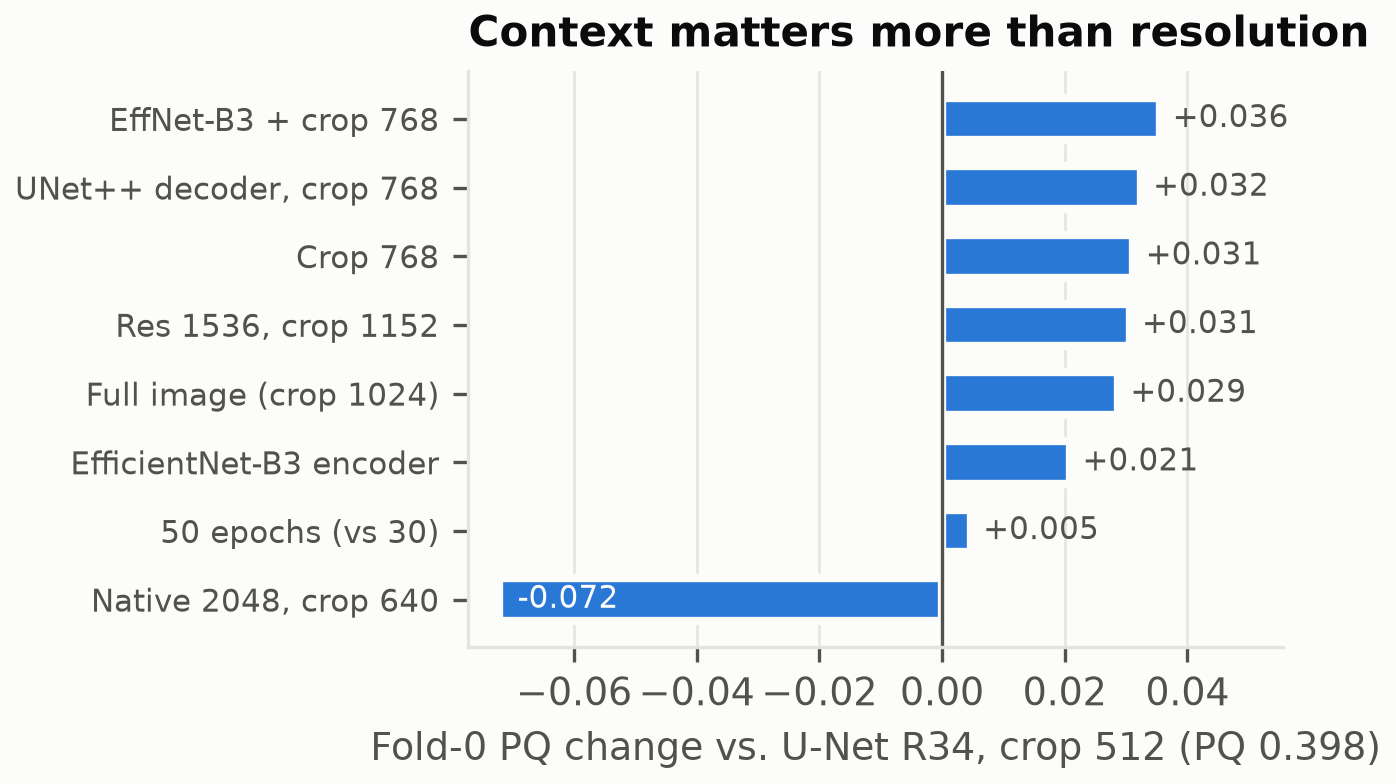
\includegraphics[width=\linewidth]{fig_ablation.png}
\caption{Single-change ablations on fold 0 (post-processing re-tuned for each).}
\label{fig:abl}
\end{figure}

\textbf{Ensemble and TTA.} ResNet34 and EfficientNet-B3 models (both 768 crops) are averaged with
equal weights, each with 8-view dihedral TTA and 5-fold averaging. A third member (UNet++ or a
1536\,px model) added $\le$0.001 and was dropped.

\textbf{Instances.} The averaged probability is thresholded at 0.3 and split into 8-connected
components. Global morphology (opening/closing/dilation) consistently hurt.

\subsection{Instance scorer}\label{sec:scorer}
For every OOF component we compute the target $y$ of Eq.~(2) and 24 features: area, bounding box,
fill and elongation; mean/max/std probability and fractions above 0.5/0.7/0.9 (threshold
persistence); number of pieces at a stricter threshold (merge indicator); perimeter ratio and
probability-edge sharpness; inner/ring intensity and contrast; distance to disk centre; image-level
counts; per-member mean probability and member disagreement. A LightGBM regressor is trained
fold-honestly and components with $\hat y>\tau$ are kept. The optimum $\tau=0.23$ sits at
$\mathrm{PQ}/2$ as Eq.~(2) predicts (Fig.~\ref{fig:tau}); the scorer adds +0.014--0.023 PQ over
the best area/probability filter on every model.

\begin{figure}[t]\centering
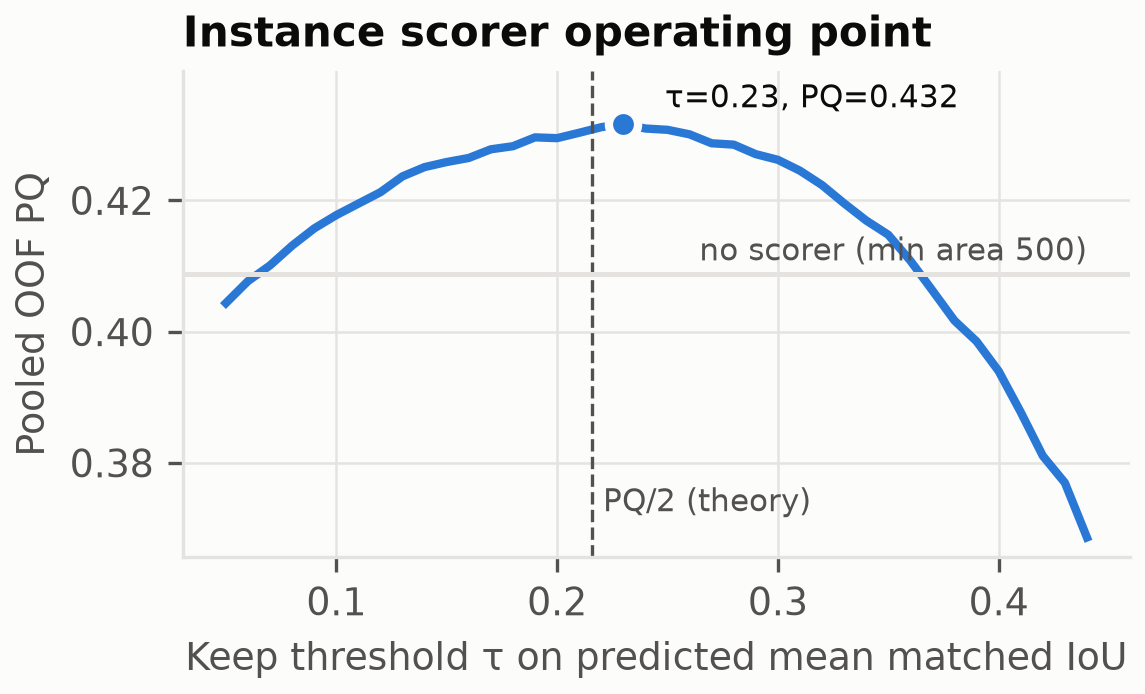
\includegraphics[width=\linewidth]{fig_tau.png}
\caption{Pooled OOF PQ vs.\ keep threshold; dashed line = PQ/2 from Eq.~(2).}
\label{fig:tau}
\end{figure}

\textbf{Submission.} Kept components are re-thresholded on the bilinearly upsampled 2048 map
(component kept if $>$50\% overlaps a selected one), giving non-overlapping masks encoded as COCO
RLE. Every file is validated (no empty or overlapping masks; RLE round-trip against GT).

\section{Results}
\begin{table}[h]\centering\small
\begin{tabular}{lcc}\toprule
Model & CV PQ & Public LB\\\midrule
R34 crop 512, components only & 0.386 & 0.33\\
R34 crop 512 + scorer & 0.401 & 0.34\\
R34 crop 768 + scorer & 0.424 & 0.35\\
R34 + EffB3 crop 768 ensemble + scorer v1 & 0.429 & 0.35\\
\quad + TTA8 + scorer v2 (final) & \textbf{0.432} & --\\\midrule
Human vs.\ human & 0.340 & --\\\bottomrule
\end{tabular}
\caption{Grouped 5-fold OOF PQ (fold std $\approx$0.01) and public leaderboard ($\approx$90 images,
two decimals). CV ranking is preserved on the leaderboard with a stable $-0.06$ offset.}
\end{table}

\begin{figure*}[t]\centering
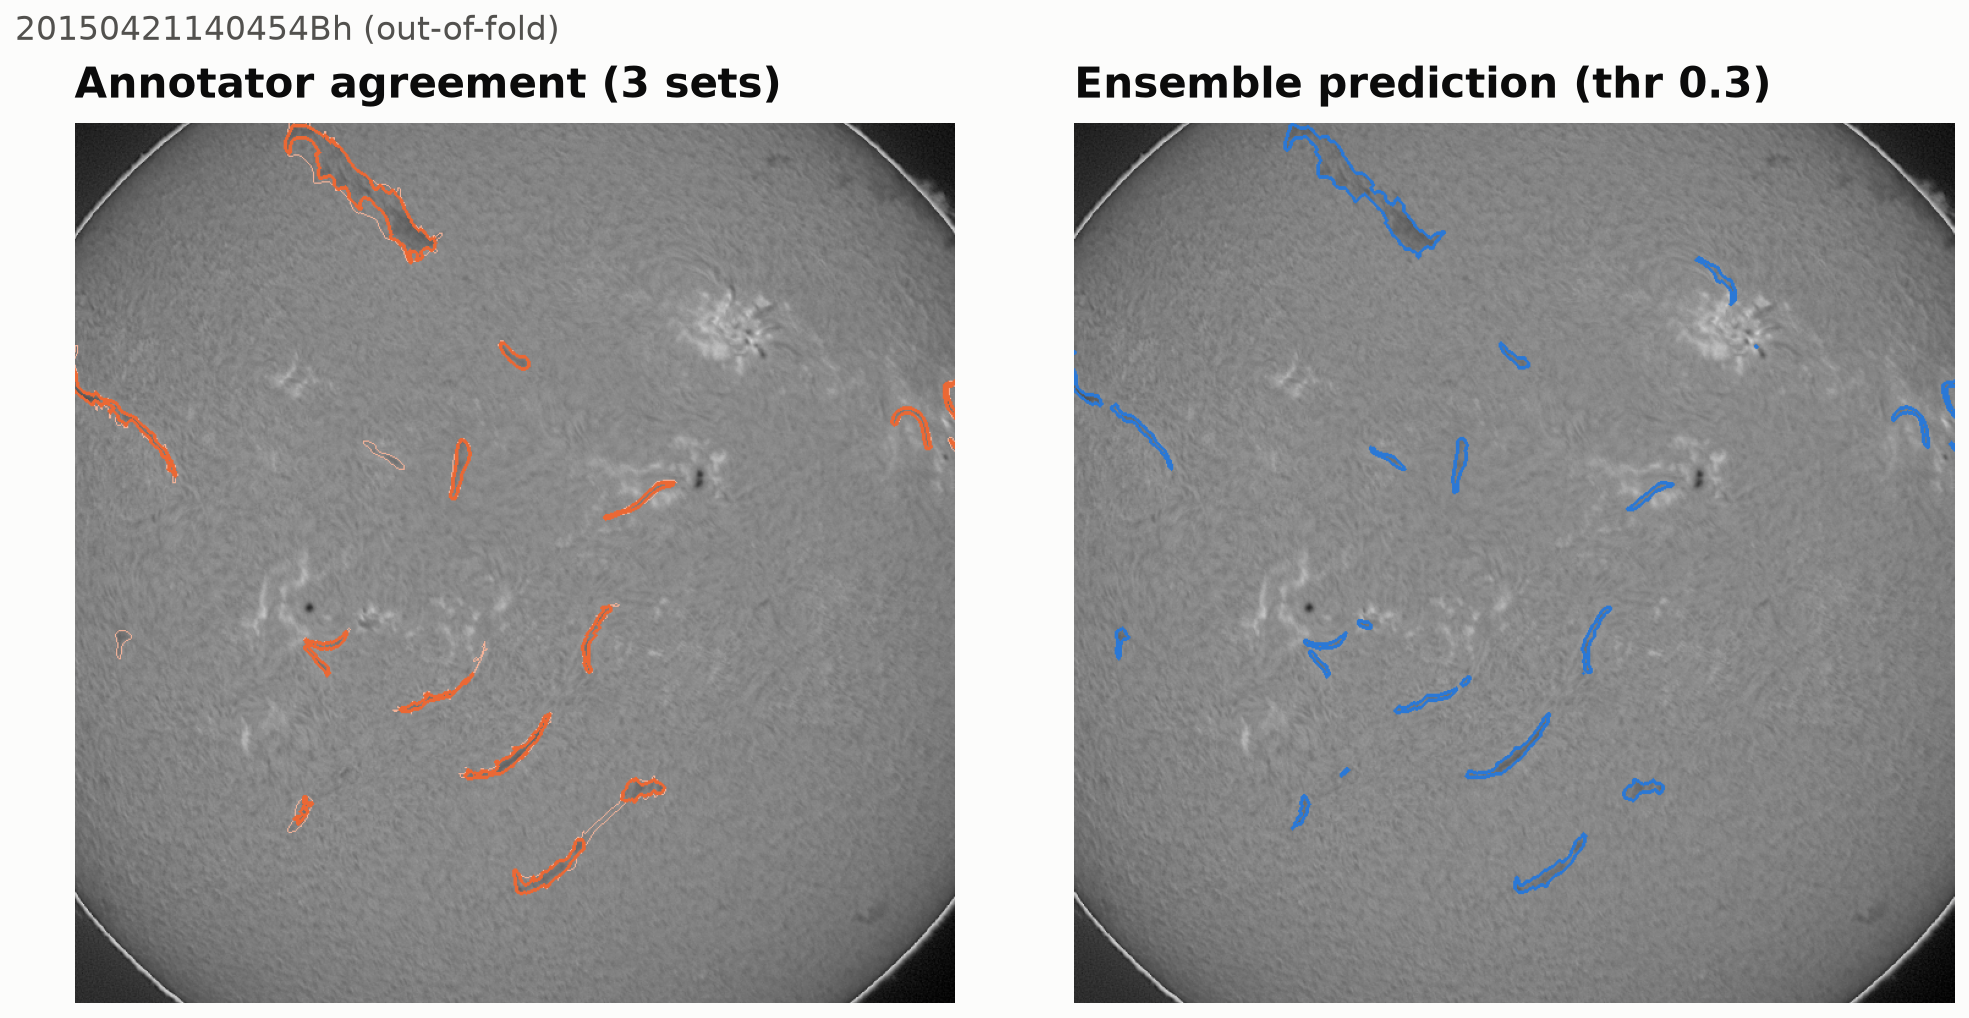
\includegraphics[width=0.85\linewidth]{fig_overlay.png}
\caption{Out-of-fold example. Left: contours where $\ge$2 of 3 annotators agree (bold) and
minority-only regions (faint). Right: ensemble prediction. Majority filaments, including thin
curved ones near active regions, are recovered as single contiguous instances.}
\label{fig:ov}
\end{figure*}

\textbf{Error analysis.} On fold 0 of the baseline, half of the false negatives are filaments
missed entirely (small, usually marked by a minority of annotators) and about a third of both
FPs and FNs are near-misses with IoU 0.3--0.5, i.e.\ boundary disagreement of the same order as
between annotators. Splits and merges account for $<$5\% of errors.

\section{Discussion and limitations}
The remaining gap is dominated by annotation ambiguity: resolution, extra architectures and longer
training each add $<$0.005 once ensembling and the scorer are in place. The scorer explicitly
optimizes for consensus filaments, which is what pooled PQ rewards; users who need every
minority-marked filament should lower $\tau$. We used no external data; the public MAGFiLO
release was deliberately excluded because it contains the test labels.

\textbf{Reproducibility.} Code, configs and a notebook running the full pipeline are in the
repository (\texttt{requirements.txt} pins all versions). Training both models takes
$\approx$12\,h on an RTX\,3050 Laptop (4\,GB); inference on the 180 test images takes minutes.

\section*{Acknowledgment}
Ideas re-implemented from public Kaggle notebooks: soft targets and instance keep threshold
(tushhaaarrrr), metric (azimahmadzadeh, host), grouped CV (dattadhebe), operating-point
selection (juanmirod).
\end{document}
